\documentclass[10pt, unicode]{beamer}
\usepackage{fontspec}
\usepackage{polyglossia}
\usepackage{graphicx}
\usepackage{float}
\usepackage{wrapfig}
\usepackage{caption}
\usepackage{subcaption}
\setdefaultlanguage{english}

\usetheme[progressbar=frametitle, numbering=fraction]{metropolis}
\useoutertheme{metropolis}
\useinnertheme{metropolis}
\usefonttheme{metropolis}
\usecolortheme{seagull}
\setsansfont{Source Sans Pro}
\captionsetup[figure]{labelformat=empty}
\captionsetup[subfigure]{labelformat=empty}

\title{Текстовый процессор для open-source движка Citrus}
\author{Студент группы Б8403а\\Куцелабский Егор Сергеевич\\Руководитель: старший 
преподаватель кафедры ИМКМ Кленин Александр Сергеевич}
\date{}

\begin{document}
    \begin{frame}
        \titlepage
        \thispagestyle{empty}
    \end{frame}
    \begin{frame}
        \frametitle{Game Forest и текст}
        \begin{figure}[h]
            \centering
            \begin{subfigure}[h]{0.59\textwidth}
                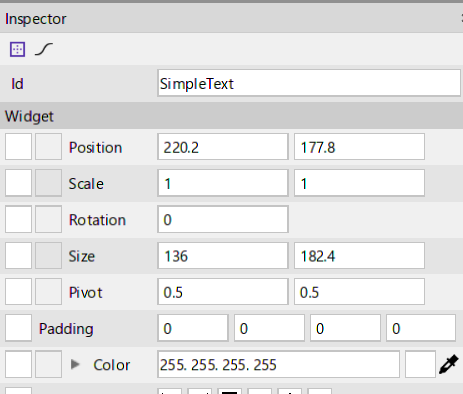
\includegraphics[width=\textwidth]{images/TangerineInterface.png}
                \caption{Часть интерфейса редактора анимаций}
            \end{subfigure}
            \begin{subfigure}[h]{0.4\textwidth}
                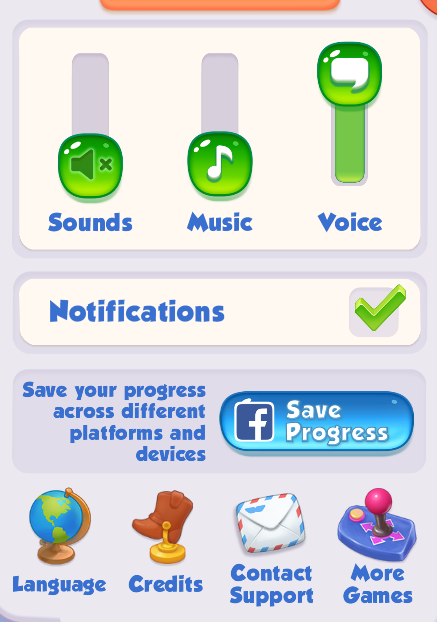
\includegraphics[width=\textwidth]{images/ToyStoryDropScreenshot.png}
                \caption{Скриншот из игры Toy Story Drop}
            \end{subfigure}
        \end{figure}
    \end{frame}
    \begin{frame}
        \frametitle{Текстовые процессоры}
        \begin{figure}[h]
            \centering
            \begin{subfigure}[h]{0.49\textwidth}
                
\includegraphics[width=\textwidth]{images/WordPic.png}
                \caption{Логотип Word}
            \end{subfigure}
            \begin{subfigure}[h]{0.49\textwidth}
                
\includegraphics[width=\textwidth]{images/SublimePic.png}
                \caption{Логотип Sublime Text}
            \end{subfigure}
        \end{figure}
    \end{frame}
    \begin{frame}
        \frametitle{Цели и задачи работы}
        Цель - создать текстовый процессор для игрового движка Citrus
        \vspace{\baselineskip}

        Задачи:
        \begin{itemize}
            \item Изучить эффективные методы представления текста
            \item Реализовать текстовый процессор
            \item Оценить выигрыш в производительности
        \end{itemize}
    \end{frame}
    \begin{frame}
        \frametitle{Структуры данных}
        \begin{figure}
            \centering
            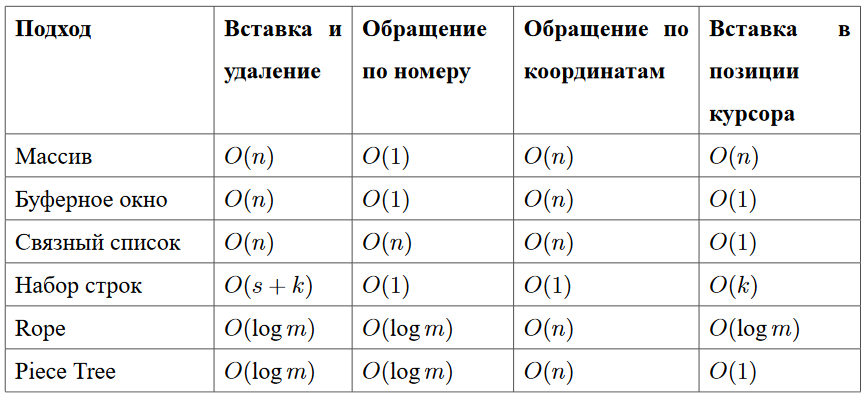
\includegraphics[width=\textwidth]{images/ComparisonTable.png}
        \end{figure}
        \begin{itemize}
            \item $n$ -- кол-во символов
            \item $s$ -- кол-во строк
            \item $k$ -- кол-во символов в строке
            \item $m$ -- высота дерева
        \end{itemize}
    \end{frame}
    \begin{frame}
        \frametitle{Функциональные требования}
        \begin{itemize}
            \item Эффективная обработка внутреннего представления текста
            \item Отрисовка текста с заданными параметрами шрифта
            \item Обработка пользовательского ввода
        \end{itemize}
    \end{frame}
    \begin{frame}
        \frametitle{Существующая версия архитектуры}
        \begin{figure}
            \centering
            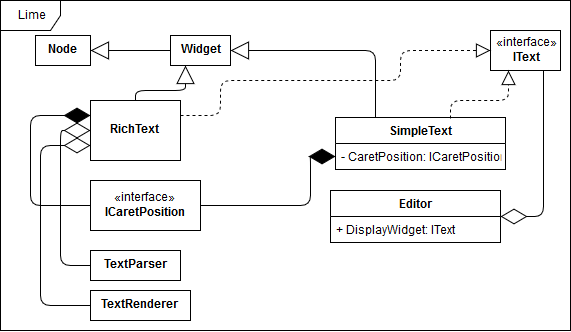
\includegraphics[width=\textwidth]{diagrams/CitrusTextSystem.png}
            \caption{Диаграмма классов текстовой системы Citrus}
        \end{figure}
    \end{frame}
    \begin{frame}
        \frametitle{Архитектура системы: представление текста}
        \begin{figure}
            \centering
            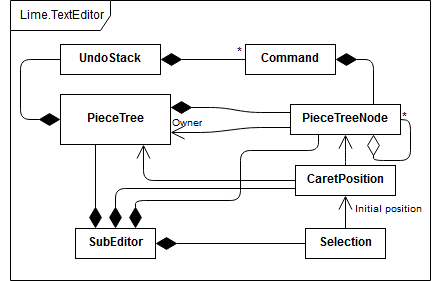
\includegraphics[width=\textwidth]{diagrams/SubEditorScheme.png}
            \caption{Диаграмма классов модуля представления текста}
        \end{figure}
    \end{frame}
    \begin{frame}
        \frametitle{Архитектура системы: отрисовка и ввод}
        \begin{figure}
            \centering
            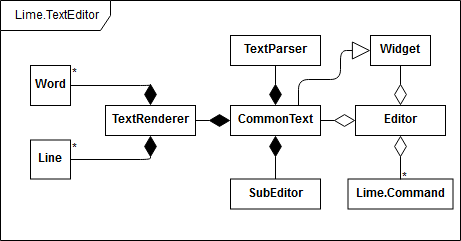
\includegraphics[width=\textwidth]{diagrams/EditorScheme.png}
            \caption{Диаграмма классов модулей отрисовки и ввода}
        \end{figure}
    \end{frame}
    \begin{frame}
        \frametitle{Piece Table}
        \begin{figure}
            \centering
            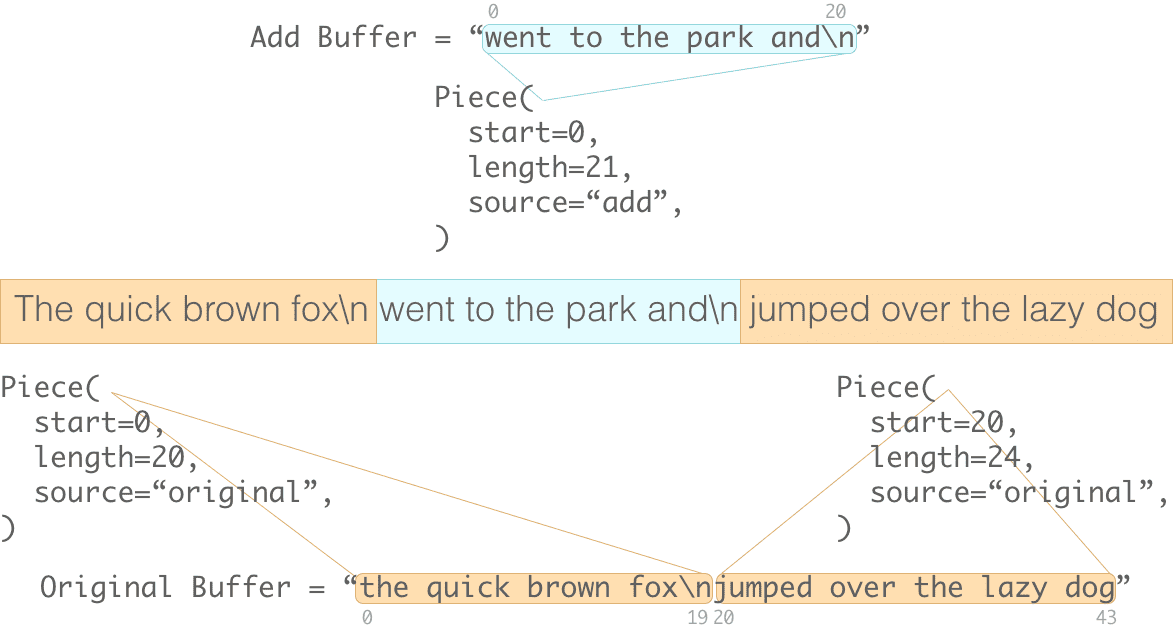
\includegraphics[width=\textwidth]{images/PieceTableExample.png}
            \caption{Пример работы Piece Table}
        \end{figure}
    \end{frame}
    \begin{frame}
        \frametitle{Splay Tree}
        \begin{figure}
            \centering
            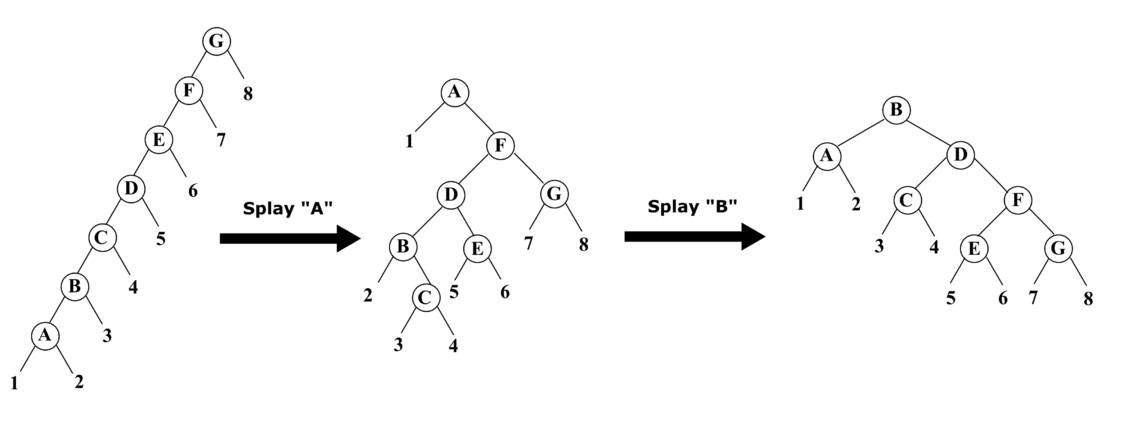
\includegraphics[width=\textwidth]{images/SplayTreeExample.png}
            \caption{Пример работы Splay Tree}
        \end{figure}
    \end{frame}
    \begin{frame}
        \frametitle{Интерфейс}
        \begin{figure}[h]
            \centering
            \begin{subfigure}[h]{0.49\textwidth}
                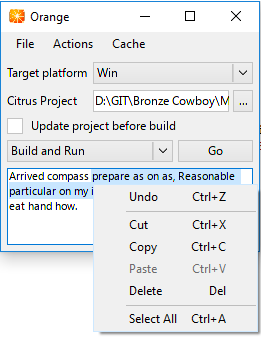
\includegraphics[width=\textwidth]{images/EditorContextMenu.png}
                \caption{Пример Editor с открытым контекстным меню в интерфейсе Citrus}
            \end{subfigure}
            \begin{subfigure}[h]{0.49\textwidth}
                
\includegraphics[width=\textwidth]{images/DecoratedBubble.png}
                \caption{Пример декорированного CommonText}
            \end{subfigure}
        \end{figure}
    \end{frame}
    \begin{frame}
        \frametitle{Тестирование: отрисовка}
        \begin{figure}
            \centering
            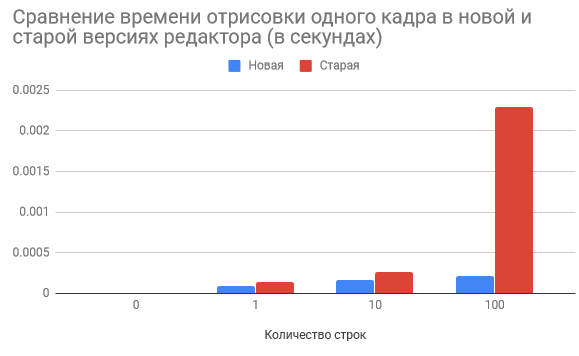
\includegraphics[width=\textwidth]{images/RenderComparisonSmall.png}
            \caption{Максимальное число строк - 100}
        \end{figure}
    \end{frame}
    \begin{frame}
        \frametitle{Тестирование: вставка}
        \begin{figure}
            \centering
            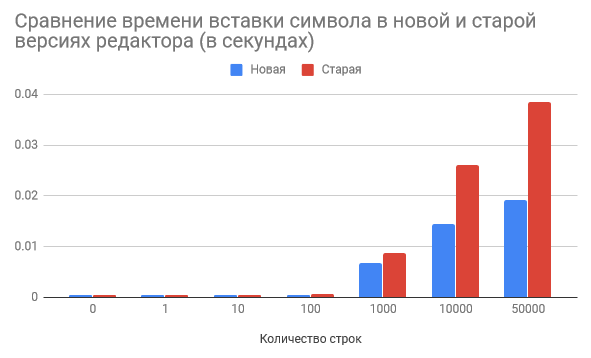
\includegraphics[width=\textwidth]{images/InsertionComparison.png}
        \end{figure}
    \end{frame}
    \begin{frame}
        \frametitle{Реализация}
        \begin{itemize}
            \item Язык программирования C\#
            \item Объём кода: 10420 добавлений, 2291 удалений, $\sim$ 149 кб (итоговый).
            \item Количество коммитов: 58
            \item Количество автотестов: 63
            \item Репозиторий: https://github.com/mrojkov/Citrus
        \end{itemize}
    \end{frame}
    \begin{frame}
        \frametitle{Заключение}
        \begin{itemize}
            \item Выполнен анализ структур данных для работы с текстом
            \item Реализована новая версия текстового процессора
            \item Реализованные модули показывают улучшение производительности по сравнению с
            предыдущей версией процессора
            \item В настоящее время код находится на этапе опытной эксплуатации
        \end{itemize}
    \end{frame}
\end{document}